\begin{prop}
\label{prop:tentMap}
$H$ is non-uniformly hyperbolic. That is, Lyapunov exponents
\[\chi (z,v) = \limn \frac{1}{n} \log||DH^n_z v|| \]
are non-zero for almost every $z \in \tor$ and tangent vector $v \neq 0$.
\end{prop}

The key ingredients of the proof were sketched out in \cite{myers_hill_exponential_2022}. We provide a more detailed treatment here as certain constructions are central to the analysis of later sections. We begin with a description of the Jacobian $DH$ and recall a decomposition of the cocycle $DH_z^n$ into blocks (Lemma \ref{lemma:itineraries}) which share an invariant expanding cone (Lemma \ref{lemma:cone}). Associating these blocks with recurrence to a region $\sigma$ then allows us to deduce non-zero Lyapunov exponents on a full measure set.

\begin{figure}
    \centering
 \begin{tikzpicture}
     \tikzmath{\e = 0.5;} 
    \node[scale=1] at (0,0) {
    \begin{tikzpicture}
    
    \fill[gray!40] (0,4-4*\e) rectangle (4-4*\e,4);
    
    \fill[gray!20] (4-4*\e,0) rectangle (4,4-4*\e);
    
    \draw (0,0) rectangle (4,4);
    \draw (4-4*\e,0) -- (4-4*\e,4);
    \draw (0,4-4*\e) -- (4,4-4*\e);
    
    
    %\node[scale=0.8] at (-0.4,4-4*\e) {$1-\eta$};
    %\node[scale=0.8] at (2,-0.3) {$\frac{1}{2}$};
    
    \node[scale=1.5] at (2-0.5*4*\e,2-0.5*4*\e) {$S_1$};
    \node[scale=1.5] at (4-0.5*4*\e,2-0.5*4*\e) {$S_2$};
    \node[scale=1.5] at (2-0.5*4*\e,4-0.5*4*\e) {$S_3$};
    \node[scale=1.5] at (4-0.5*4*\e,4-0.5*4*\e) {$S_4$};
    
    \end{tikzpicture}
    };
    \node[scale=1] at (-5,0) {
    \begin{tikzpicture}
    
    \filldraw[fill=gray!40] (0, {4*(1-\e+\e*\e)}) -- ({4*(1-\e)},4) -- (0,4) --  (0, {4*(1-\e+\e*\e)});
    
    \filldraw[fill=gray!40] (4,4) -- (0,{4*(1-\e)}) -- ({4*(1-\e)},{4*(1-\e)}) -- (4, {4*(1-\e+\e*\e)}) -- (4,4);
    
    \filldraw[fill=gray!20] ({4*(1-\e)},{4*(1-\e)}) -- (4,{4*(1-\e)}) -- (4, {4*(1-\e)^2}) -- ({4*(1-\e)},{4*(1-\e)});
    
    \filldraw[fill=gray!20] (0,{4*(1-\e)}) -- (4,0) -- ({4*(1-\e)},0) -- (0, {4*(1-\e)^2}) -- (0,{4*(1-\e)});
    
    \draw (0,0) rectangle (4,4);

    %\node[scale=0.8] at (-0.2,4-4*\e) {$\frac{1}{2}$};
    %\node[scale=0.8] at (4-4*\e,-0.2) {$1-\eta$};
    
    %\node[scale=0.8] at (4.7, {4*(1-\e+\e*\e)}) {$1-\eta+\eta^2$};
       % \node[scale=0.8] at (-0.2, {4*(1-\e+\e*\e)}) {$\frac{3}{4}$};
    %\node[scale=0.8] at (4.55, {4*(1-\e)^2}) {$(1-\eta)^2$};
        %\node[scale=0.8] at (-0.2, {4*(1-\e)^2}) {$\frac{1}{4}$};
        
    %\node[scale=0.8] at (2,-0.3) {$\frac{1}{2}$};    
    \node at (2-0.5*4*\e,2-0.5*4*\e) {$A_2$};
    \node at (3.5,1.6) {$A_2$};
    \node at (3.5,2.4) {$A_4$};
    
    \node at (2,1.5) {$A_1$};
    \node at (2-0.5*4*\e,2+0.5*4*\e) {$A_4$};

    \node at (2,2.5) {$A_3$};
    \node at (0.4,3.6) {$A_3$};
    \node at (0.4,0.4) {$A_1$};
    \end{tikzpicture}
    };
    
    \node[scale=1] at (5,0) {
    \begin{tikzpicture}
    
    \filldraw[fill = gray!40] (0,4-4*\e) -- ({4*\e*(1-\e)},4) -- (0,4) -- (0,4-4*\e);
    \filldraw[fill = gray!40] (0,0) -- (4-4*\e,4) -- (4-4*\e,4-4*\e) -- ({4*\e*(1-\e)},0) -- (0,0);
    
    \filldraw[fill=gray!20] (4-4*\e,0) -- (4-4*\e,4-4*\e) -- (4-4*\e*\e,0) -- (4-4*\e,0);
    \filldraw[fill=gray!20] (4,0) -- (4-4*\e,4) -- (4-4*\e*\e,4)-- (4,4-4*\e) -- (4,0);
    
    \draw (0,0) rectangle (4,4);
    % \draw (4-4*\e,0) -- (4-4*\e,4);
    % \draw (0,4-4*\e) -- (4,4-4*\e);
    
    % \node[scale=0.8] at ({4*\e*(1-\e)},-0.2) {$x_1$};
    % \node[scale=0.8] at ({4*(1-\e*\e)},-0.2) {$x_2$};
    
    %\node[scale=0.8] at (-0.4,4-4*\e) {$1-\eta$};
    %\node[scale=0.8] at (4-4*\e,-0.2) {$1-\eta$};

    \node at (1.5,2) {$A_3'$};
    \node at (1.7,0.5) {$A_1'$};
    \node at ({0.4*4*(1-\e)},2.5) {$A_1'$};  
    \node at (0.3,3.5) {$A_3'$};

    \node at (4-1.5,2) {$A_4'$};
    \node at (4-1.7,0.5) {$A_2'$};
    \node at ({4-0.4*4*(1-\e)},2.5) {$A_2'$};  
    \node at (4-0.3,3.5) {$A_4'$};

    \end{tikzpicture}
    };
    
\draw[->, thick] (-2.7,0) -- (-2.2,0); 
    \node[scale=1.5] at (-2.45,0.4) {$F$};
    \draw[->, thick] (2.2,0) -- (2.7,0); 
    \node[scale=1.5] at (2.45,0.4) {$G$};
    
    \end{tikzpicture}
    \caption{A partition of the torus into four rectangles $S_j$, and their preimages $A_j$, $A_j'$ under $F,G^{-1}$.}
        \label{fig:firstPartitions}
\end{figure}

Partition the torus into the four squares $S_j$ shown in Figure \ref{fig:firstPartitions}. The Jacobian $DH$ is then constant on the preimages $A_j=F^{-1}(S_j)$, given by the matrix $M_j$ where
\[ M_1 = \begin{pmatrix} 1 & 2 \\ 2 & 5\end{pmatrix}, \quad M_2 = \begin{pmatrix} 1 & 2 \\ -2 & -3\end{pmatrix}, \quad M_3 = \begin{pmatrix} 1 & -2 \\ 2 & -3\end{pmatrix}, \quad M_4 = \begin{pmatrix} 1 & -2 \\ -2 & 5\end{pmatrix}, \]
undefined on the singularity set $\mathcal{D} = \cup_j \partial A_j$. Letting $X'$ denote the full measure set $\tor \setminus \cup_{i \geq 0} H^{-i}(\mathcal{D})$, the $n$-step itinerary
\[  A_{j_1}, A_{j_2}, A_{j_3}, \dots, A_{j_n},\]
is well defined for any $z \in X'$. The related cocycle $DH_z^n$ given by
\[ DH_z^n = M_{j_n} \dots M_{j_3} M_{j_2}  M_{j_1}\]
with each $j_k \in \{ 1,2,3,4 \}$. Our aim is to decompose any cocycle into hyperbolic matrices which share an invariant expanding cone.
Note that while $M_1$ and $M_4$ are hyperbolic, $M_2$ and $M_3$ are not. Hence when $M_2$ or $M_3$ appear in a cocycle at $M_{j_k}$, we must combine them with its neighbouring matrices $M_{j_{k+l}},\dots,M_{j_{k+2}}, M_{j_{k+1}}$ for some $l \in \mathbb{N}$.

Consider the countable family of matrices 
\[\mathcal{M} = \{ M_1, M_4,  M_1M_2^n, M_3M_2^n, M_4M_2^n, M_1M_3^n, M_2M_3^n, M_4M_3^n\} \]
with $n\in\mathbb{N}$. Similarly define 
\[\mathcal{M}' = \{ M_1^{-1}, M_4^{-1},  M_1^{-1}M_2^{-n}, \dots, M_4^{-1}M_3^{-n}\}.\]
It was shown in \cite{myers_hill_exponential_2022} that:

\begin{lemma}
\label{lemma:itineraries}
At almost every $z$, the cocycle $DH_z^n$ can be decomposed into blocks from $\mathcal{M}$.
\end{lemma}

The result essentially follows from the fact that essentially no orbits get trapped in $A_3$,
\begin{equation}
    \label{eq:escapeA3statement}
    \limn \mu\left( \{ z \in A_3 \, | \, H^i(z) \in A_3 \text{ for all } 0 \leq i \leq n-1  \}\right) = 0,
\end{equation}
and the equivalent statement for $A_2$. An entirely analogous argument, considering escapes from $A_2'$ and $A_3'$ under $H^{-1}$, gives that at a.e. $z$ the cocycle $DH_z^{-n}$ can be decomposed into blocks from $\mathcal{M}'$. 

\begin{lemma}
\label{lemma:cone}
The matrices in $\mathcal{M}$ admit an invariant expanding cone $\mathcal{C}$.
\end{lemma}

\begin{proof}
Parameterise the tangent space by $(v_1,v_2)^T\in \mathbb{R}^2$. The lemma was shown in \cite{myers_hill_exponential_2022} using the cone $C = \{(v_1,v_2)\neq 0 \,|\, |v_2| \geq \phi \, |v_1|\}$ where $\phi$ is the golden ratio $(1+\sqrt{5})/2$. Here we define a slightly wider cone $\mathcal{C} = \{(v_1,v_2)\neq 0 \,|\, |v_2| \geq  \varphi \, |v_1|\}$, $\varphi = 21/13$, which still contains all the unstable eigenvectors of matrices in $\mathcal{M}$ and none of the stable eigenvectors. Hence $\mathcal{C}$ is invariant and one can verify that it is also expanding (minimum expansion factors are calculated later in Table \ref{tab:tab2}, in particular the minimum expansion of a matrix $M$ over $\mathcal{C}$ under the $\| \cdot\|_\infty$ norm is given by $\min_\pm K_\pm(M)$). 
%Defining $\mathcal{C}' = \{(v_1,v_2)\neq 0 \,|\, |v_1| \geq \varphi \, |v_2|\}$, the second claim follows by an entirely analogous argument.
\end{proof}


\subsubsection*{Recurrence to $\sigma$}

\begin{figure}
    \centering
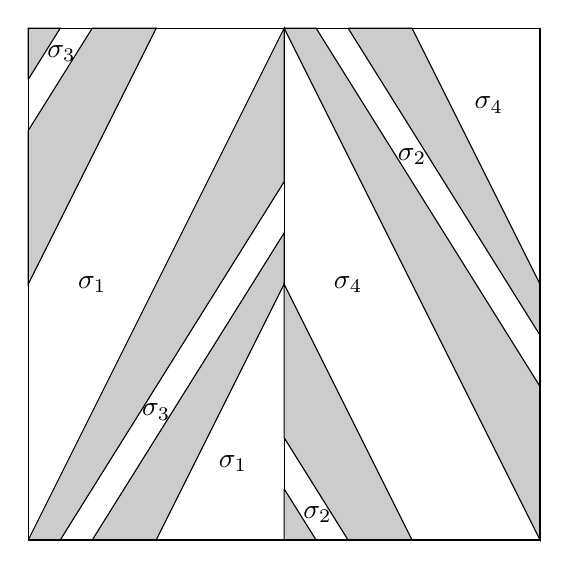
\begin{tikzpicture}[scale=0.65]
    
    \draw (5,0) -- (5,10);
    \filldraw[fill=gray!40] (0,8) -- (10/8,10) -- (2.5,10) -- (0,5) -- (0,8);
      \filldraw[fill=gray!40] (0,9) -- (0,10) -- (10/16,10) -- (0,9);
      \filldraw[fill=gray!40] (0,0) -- (5,10) -- (5,7) -- (10/16,0) -- (0,0);
      \filldraw[fill=gray!40] (10/8,0) -- (2.5,0) -- (5,5) -- (5,6) -- (10/8,0) ;
      \filldraw[fill=gray!40] (5,2) -- (50/8,0) -- (7.5,0) -- (5,5) -- (5,2);
      \filldraw[fill=gray!40] (5,1) -- (5,0) -- (90/16,0) -- (5,1);
      \filldraw[fill=gray!40] (5,10) -- (10,0) -- (10,3) -- (90/16,10) -- (5,10);
      \filldraw[fill=gray!40] (50/8,10) -- (7.5,10) -- (10,5) -- (10,4) -- (50/8,10);
 
     \node at (0.65,9.5) {$\sigma_3$};
     \node at (1.25,5) {$\sigma_1$};
     \node at (2.5,2.5) {$\sigma_3$};
     \node at (4,1.5) {$\sigma_1$};
     
     \node at (0.65+5,10-9.5) {$\sigma_2$};
     \node at (1.25+5,5) {$\sigma_4$};
     \node at (2.5+5,10-2.5) {$\sigma_2$};
    \node  at (4+5,10-1.5) {$\sigma_4$};
     \draw(0,0) rectangle (10,10);
    \end{tikzpicture}
    \hspace{2em}
    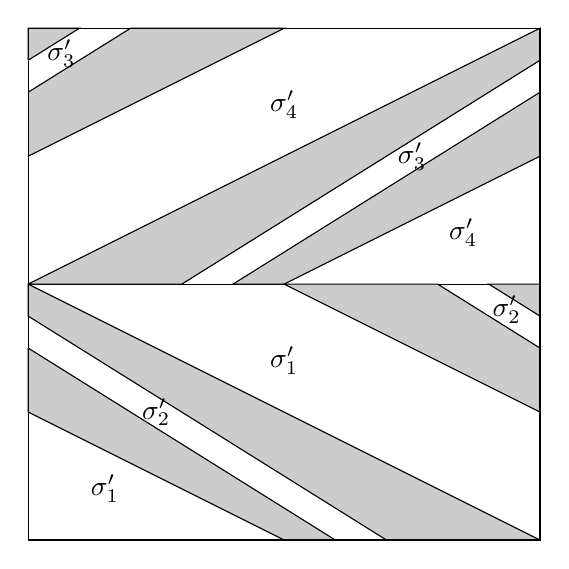
\begin{tikzpicture}[scale=0.65]
    
    \draw (0,5) -- (10,5);
    \filldraw[fill=gray!40] (0,150/16) -- (0,10) -- (1,10) -- (0,150/16);
      \filldraw[fill=gray!40] (0,70/8) -- (2,10) -- (5,10) -- (0,7.5);
      \filldraw[fill=gray!40] (0,5) -- (10,10) -- (10,150/16) -- (3,5) -- (0,5);
      \filldraw[fill=gray!40] (10,70/8) -- (10,7.5) -- (5,5) -- (4,5) -- (10,70/8) ;
   
     \filldraw[fill=gray!40] (10,150/16-5) -- (10,10-5) -- (10-1,10-5) -- (10,150/16-5);
      \filldraw[fill=gray!40] (10,70/8-5) -- (10-2,10-5) -- (10-5,10-5) -- (10,7.5-5);
      \filldraw[fill=gray!40] (10,5-5) -- (0,10-5) -- (0,150/16-5) -- (10-3,5-5) -- (10,5-5);
      \filldraw[fill=gray!40] (0,70/8-5) -- (0,7.5-5) -- (10-5,5-5) -- (10-4,5-5) -- (0,70/8-5) ;   
 
     \node at (0.65,9.5) {$\sigma_3'$};
     \node at (5,8.5) {$\sigma_4'$};
     \node at (7.5,7.5) {$\sigma_3'$};
     \node at (8.5,6) {$\sigma_4'$};
     
     \node at (10-0.65,9.5-5) {$\sigma_2'$};
     \node at (10-5,8.5-5) {$\sigma_1'$};
     \node at (10-7.5,7.5-5) {$\sigma_2'$};
     \node at (10-8.5,6-5) {$\sigma_1'$};

    %  \node at (0.65+5,10-9.5) {$\sigma_2$};
    %  \node at (1.25+5,5) {$\sigma_4$};
    %  \node at (2.5+5,10-2.5) {$\sigma_2$};
    % \node  at (4+5,10-1.5) {$\sigma_4$};
     \draw(0,0) rectangle (10,10);
    \end{tikzpicture}
   
     \caption{Partitions of the return sets $\sigma,\sigma'$ (white) for $H,H^{-1}$ into four sets $\sigma_j \subset H(A_j)$, $\sigma_j' \subset H^{-1}(A_j')$.  \label{fig:sigmaPartition}}
\end{figure}

Define $\sigma$ as the union of the sets $\sigma_1 = H(A_1)$, $\sigma_2 = H(A_2 \cap H(A_3))$, $\sigma_3 = H(A_3 \cap H(A_2)$, $\sigma_4 = H(A_4)$. By construction, any orbit escaping $A_2,A_3$ or passing through $A_1,A_4$ must pass through $\sigma$. The return map $H_\sigma : \sigma \to \sigma$, $z \mapsto H^R(z)$ where $R = R(z;H,\sigma)$, is well defined at $\mu$-almost every $z \in \sigma$ by (\ref{eq:escapeA3statement}) and the equivalent statement for $A_2$. We similarly define $\sigma' = \cup_j \sigma_j'$ using the $A_j'$ and the return map $H^{-1}_{\sigma'}:\sigma' \rightarrow \sigma'$ for $H^{-1}$. The sets $\sigma,\sigma'$ are shown as the unshaded regions in Figure \ref{fig:sigmaPartition}.

We begin by identifying the points in $\sigma$ with return time 1, i.e. $H^{-1}(\sigma) \cap \sigma$. The preimages of $\sigma_1, \sigma_4$ are simply $A_1$, $A_4$ and by definition we have $H^{-1}(\sigma_2) = A_2 \cap H(A_3)$ so that $H^{-1}(\sigma_2) \cap \sigma = A_2 \cap \sigma_3 := \varsigma_3$ and similarly $H^{-1}(\sigma_3) \cap \sigma = A_3 \cap \sigma_2 := \varsigma_2$. See Figure \ref{fig:returnTime1} for an illustration. 

\begin{figure}
    \centering
    \subfigure[][]{
    \label{fig:returnTime1}
    
    \definecolor{tomato}{RGB}{255, 99, 71}
    \definecolor{teal}{RGB}{95, 158, 160} 
    
     \begin{tikzpicture}[scale=0.7]
    
    \clip (0,0) rectangle (10,10);
    
    \draw (0,5) -- (10,5);
    
    %\draw (0,0) rectangle (10,10);
    \draw (0,10) -- (10,10);
    \draw (5,0) -- (10,0);

    \filldraw[fill=tomato!80] (0,5) -- (5,5) -- (10,2.5) -- (10,0) -- (0,5);
    \filldraw[fill=tomato!80] (0,2.5) -- (5,0) -- (0,0) -- (0,2.5);
    
    \filldraw[fill=tomato!80] (0,5) -- (10,10) -- (5,10) -- (0,7.5) -- (0,5);
    \filldraw[fill=tomato!80] (5,5) -- (10,5) -- (10,7.5) -- (5,5);

    \begin{scope}
    \clip (0,0) -- (5,10) -- (5,5) -- (2.5,0) -- (0,0);
    \filldraw[fill=teal!80] (0,5) -- (10,0) -- (5,0) -- (0,2.5) -- (0,5);
    \end{scope}
    
    \begin{scope}
    \clip (10,0) -- (5,10) -- (7.5,10) -- (10,5) -- (10,0);
    \filldraw[fill=teal!80] (0,5) -- (10,10) -- (10,7.5) -- (5,5) -- (0,5);
    \end{scope}
    
  
      \filldraw[fill=gray!80] (0,8) -- (10/8,10) -- (2.5,10) -- (0,5) -- (0,8);
      \filldraw[fill=gray!80] (0,9) -- (0,10) -- (10/16,10) -- (0,9);
      \filldraw[fill=gray!80] (0,0) -- (5,10) -- (5,7) -- (10/16,0) -- (0,0);
      \filldraw[fill=gray!80] (10/8,0) -- (2.5,0) -- (5,5) -- (5,6) -- (10/8,0) ;
      
      \filldraw[fill=gray!80] (5,2) -- (50/8,0) -- (7.5,0) -- (5,5) -- (5,2);
      \filldraw[fill=gray!80] (5,1) -- (5,0) -- (90/16,0) -- (5,1);
      \filldraw[fill=gray!80] (5,10) -- (10,0) -- (10,3) -- (90/16,10) -- (5,10);
      \filldraw[fill=gray!80] (50/8,10) -- (7.5,10) -- (10,5) -- (10,4) -- (50/8,10);

    \draw (0,0) -- (0,3);
    \draw (0,4) -- (0,5);
    
    \draw (10,5) -- (10,8);
    \draw (10,9) -- (10,10);
    \node at (2.5,2.5) {$\varsigma_3$};
    \node at (7.5,7.5) {$\varsigma_2$};
    \end{tikzpicture}
    
 
    }
         \subfigure[][]{
    \label{fig:HSigma}
    
    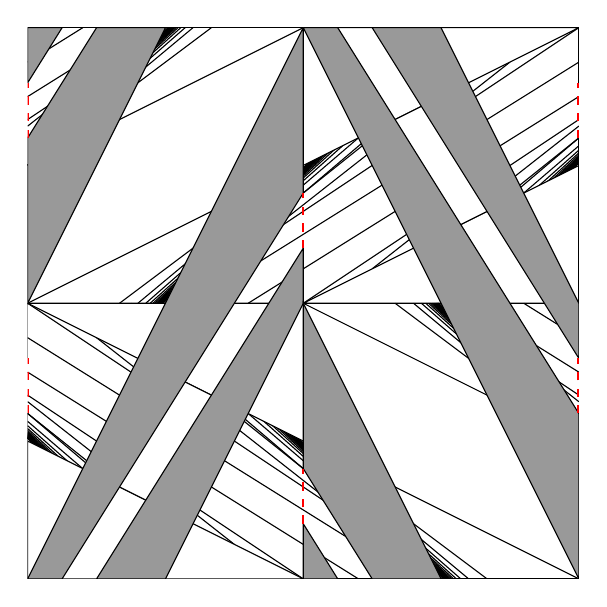
\begin{tikzpicture}[scale=0.7]
    
    \clip (0,0) rectangle (10,10);
    
    \draw (0,5) -- (10,5);
    
    %\draw (0,0) rectangle (10,10);
    \draw (0,10) -- (10,10);
    \draw (5,0) -- (10,0);
    
        
        \foreach \k in {1,...,25}{
        % Blue in R3
        \draw ({ (2*\k+2)*(7.5-7.5)/(2*\k+1)  }, { 7.5 })--({ (2*\k+2)*(10-7.5)/(2*\k+1)  }, { 10 });
        \draw ({ 5+ (2*\k+2)*(5-7.5)/(2*\k+1)  }, { 5 })--({ 5+ (2*\k+2)*(7.5-7.5)/(2*\k+1) }, { 7.5 });
        % Red in A3/A4
        \draw({ 2.5 + (2*\k+1)*(5-5)/(2*\k)  }, { 5 })--({ 2.5 + (2*\k+1)*(10-5)/(2*\k)  }, { 10 });
        \draw ({ 12.5 + (2*\k+1)*(5-10)/(2*\k)  }, { 5 }) -- ({ 12.5 + (2*\k+1)*((30*\k+20)/(4*\k+2)-10)/(2*\k)  }, { (30*\k+20)/(4*\k+2) });
        }
        
        % Red green, n=2
        \draw (30/4,70/8) -- (4,6);
        \draw (70/8,150/16) -- (7,8);
        % Symmetries...
        \draw (15-30/4,15-70/8) -- (15-5,15-190/28);
        \draw (15-70/8,15-150/16) -- (15-7,15-8);
        % Top left corner...
        %% Red red
        \draw (2.5,10) -- (0 , 50/6);
        %% Red green
        \draw (1,9) -- (0,15-190/28);
        
        
        % Red green, n=3
        \draw (5,7)--(90/14,230/28);
        % Symmetry
        \draw (15-5,15-7)--(15-90/14,15-230/28);
        
        \filldraw[fill=white] (0,5) -- (10,10) -- (5,10) -- (0,7.5) -- (0,5);
        \filldraw[fill=white] (5,5) -- (10,7.5) -- (10,5) -- (5,5);
        
        
        % Red green, n=1
        \draw (0,150/16) -- (1,10);
        \draw (0,70/8) -- (2,10);
        \draw (10,150/16) -- (3,5);
        \draw (10,70/8) -- (4,5);
      
       % We can get other sing set lines by reflecting in x=1/2 then translating x->x-1/2
       \foreach \k in {1,...,25}{
        % Blue in R3
        \draw ({10- (2*\k+2)*(7.5-7.5)/(2*\k+1)  }, { 7.5-5 })--({10- (2*\k+2)*(10-7.5)/(2*\k+1)  }, { 10-5 });
        \draw ({ 5 - (2*\k+2)*(5-7.5)/(2*\k+1)  }, { 5-5 })--({ 5 - (2*\k+2)*(7.5-7.5)/(2*\k+1)  }, { 7.5-5 });
        % Red in A3/A4
        \draw ({ 7.5 - (2*\k+1)*(5-5)/(2*\k)  }, { 5-5 })--({ 7.5- (2*\k+1)*(10-5)/(2*\k)  }, { 10-5 });
        \draw ({ -2.5 - (2*\k+1)*(5-10)/(2*\k)  }, { 5-5 }) -- ({ -2.5 - (2*\k+1)*((30*\k+20)/(4*\k+2)-10)/(2*\k)  }, { (30*\k+20)/(4*\k+2) -5 });
        }
        
        % Red green, n=2
        \draw (10-30/4,70/8-5) -- (10-4,6-5);
        \draw (10-70/8,150/16-5) -- (10-7,8-5);
        % Symmetries...
        \draw (-5+30/4,15-70/8-5) -- (0,15-190/28-5);
        \draw (-5+70/8,15-150/16-5) -- (-5+7,15-8-5);
        % Top left corner...
        %% Red red
        \draw (10-2.5,10-5) -- (10, 50/6-5);
        %% Red green
        \draw (10-1,9-5) -- (10,15-190/28-5);
        
        
        % Red green, n=3
        \draw (10-5,7-5)--(10-90/14,230/28-5);
        % Symmetry
        \draw (0,15-7-5)--(-5+90/14,15-230/28-5);
        
        \filldraw[fill=white] (10,0) -- (0,5) -- (5,5) -- (10,2.5) -- (10,0);
        \filldraw[fill=white] (0,0) -- (5,0) -- (0,2.5) -- (0,0);
        
        
        % Red green, n=1
        \draw (10,150/16-5) -- (10-1,10-5);
        \draw (10,70/8-5) -- (10-2,10-5);
        \draw (0,150/16-5) -- (10-3,5-5);
        \draw (0,70/8-5) -- (10-4,5-5);
       
   \begin{scope}
    \clip (0,0) -- (5,10) -- (5,5) -- (2.5,0) -- (0,0);
    \filldraw[fill=white] (0,5) -- (10,0) -- (5,0) -- (0,2.5) -- (0,5);
    \end{scope}
    
    \begin{scope}
    \clip (10,0) -- (5,10) -- (7.5,10) -- (10,5) -- (10,0);
    \filldraw[fill=white] (0,5) -- (10,10) -- (10,7.5) -- (5,5) -- (0,5);
    \end{scope}
       
       
       
       
      \filldraw[fill=gray!80] (0,8) -- (10/8,10) -- (2.5,10) -- (0,5) -- (0,8);
      \filldraw[fill=gray!80] (0,9) -- (0,10) -- (10/16,10) -- (0,9);
      \filldraw[fill=gray!80] (0,0) -- (5,10) -- (5,7) -- (10/16,0) -- (0,0);
      \filldraw[fill=gray!80] (10/8,0) -- (2.5,0) -- (5,5) -- (5,6) -- (10/8,0) ;
      
      \filldraw[fill=gray!80] (5,2) -- (50/8,0) -- (7.5,0) -- (5,5) -- (5,2);
      \filldraw[fill=gray!80] (5,1) -- (5,0) -- (90/16,0) -- (5,1);
      \filldraw[fill=gray!80] (5,10) -- (10,0) -- (10,3) -- (90/16,10) -- (5,10);
      \filldraw[fill=gray!80] (50/8,10) -- (7.5,10) -- (10,5) -- (10,4) -- (50/8,10);

    \draw (0,0) -- (0,3);
    \draw (0,4) -- (0,5);
    
    \draw (10,5) -- (10,8);
    \draw (10,9) -- (10,10);

    \draw[red, dashed, very thick] (0,3)--(0,4);
    \draw[red, dashed, very thick] (0,8)--(0,9);
    \draw[red, dashed, very thick] (10,3)--(10,4);
    \draw[red, dashed, very thick] (10,8)--(10,9);

    \draw[red, dashed, thick] (5,1) -- (5,2);
    \draw[red, dashed, thick] (5,6) -- (5,7);

    \end{tikzpicture}
    }
    
    \caption{Part (a) shows the portions of $\sigma$ (red, blue) with return time 1 to $\sigma$. Points in the white region have return times of 2 or more. Part (b) shows the singularity set $\mathcal{S}$ for the return map $H_\sigma$. Red dashed lines denote the shared boundaries of the $\sigma_j$.}
    \label{fig:sigmaSingSet}
\end{figure}

\begin{figure}
    \centering
    
         \subfigure[][]{
    \label{fig:escapeTimes}
    
    
    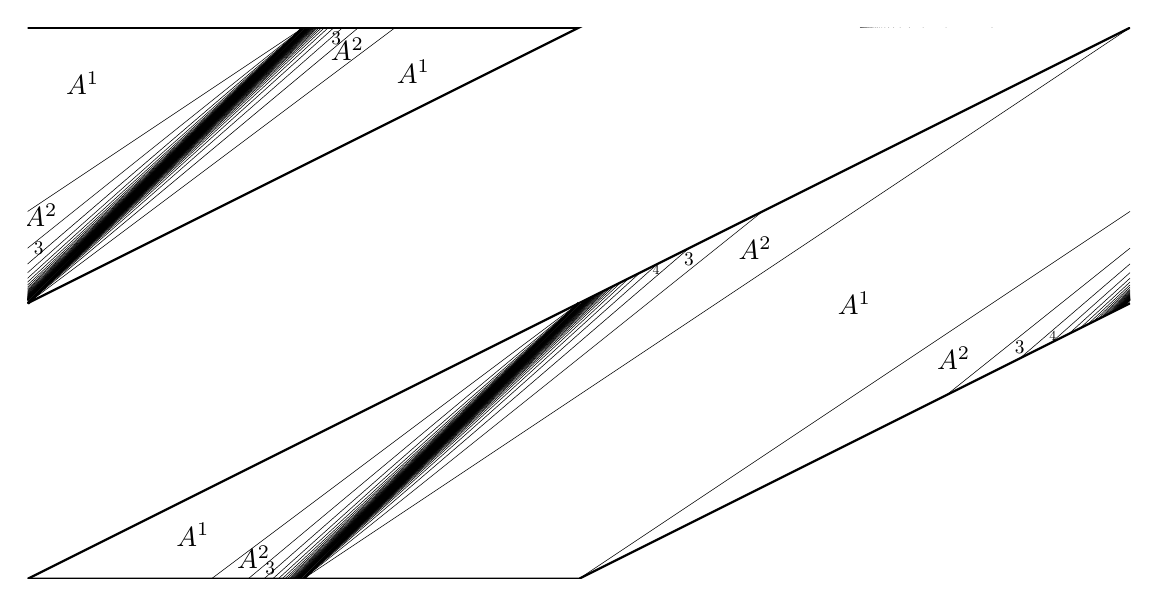
\begin{tikzpicture}[scale=1.4]
    
    \clip (0,5) rectangle (10,10);
    
    %\draw (0,5) -- (5,5);
    
    %\draw (0,10) -- (5,10);
        
        \foreach \k in {1,...,45}{
        % Blue in R3
        \draw[very thin] ({ (2*\k+2)*(7.5-7.5)/(2*\k+1)  }, { 7.5 })--({ (2*\k+2)*(10-7.5)/(2*\k+1)  }, { 10 });
        \draw[very thin] ({ 5+ (2*\k+2)*(5-7.5)/(2*\k+1)  }, { 5 })--({ 5+ (2*\k+2)*(7.5-7.5)/(2*\k+1) }, { 7.5 });
        % Red in R3/R4
        \draw[very thin] ({ 2.5 + (2*\k+1)*(5-5)/(2*\k)  }, { 5 })--({ 2.5 + (2*\k+1)*(10-5)/(2*\k)  }, { 10 });
        
         \draw[very thin] ({ 2.5  }, { 10 })--({ 2.5 - (2*\k+1)*(10-5)/(2*\k)  }, { 5 });
        
        \draw[very thin] ({ 12.5 + (2*\k+1)*(5-10)/(2*\k)  }, { 5 }) -- ({ 12.5 + (2*\k+1)*((30*\k+20)/(4*\k+2)-10)/(2*\k)  }, { (30*\k+20)/(4*\k+2) });
        }

        
        \fill[fill=white] (0,5) -- (10,10) -- (5,10) -- (0,7.5);
        \fill[fill=white] (10,5) -- (5,5) -- (10,7.5);
        
        \draw[thick] (0,10) -- (5,10) -- (0,7.5);
        \draw[thick] (0,5) -- (10,10);
        \draw[thick] (0,5) -- (5,5) -- (10,7.5); 
        
        
        \node at (7.5,7.5) {$A^1$};
        \node at (6.6,8) {$A^2$};
        \node[scale=0.7] at (6,7.9) {$3$};
        \node[scale=0.5] at (5.7,7.8) {$4$};
        
         \node at (0.5,9.5) {$A^1$};
        \node at (0.12,8.3) {$A^2$};
        \node[scale=0.7] at (0.1,8) {$3$};
        
        \node at (15-6.6,15-8) {$A^2$};
        \node[scale=0.7] at (15-6,15-7.9) {$3$};
        \node[scale=0.5] at (15-5.7,15-7.8) {$4$};
        
        
        
        \node at (3.5,9.6) {$A^1$};
        \node at (2.9,9.8) {$A^2$};
        \node[scale=0.7] at (2.8,9.9) {$3$};
        
        
        \node at (5-3.5,15-9.6) {$A^1$};
        \node at (5-2.95,15-9.8) {$A^2$};
        \node[scale=0.7] at (5-2.8,15-9.9) {$3$};
        
        \draw[very thick] (0,7.5) -- (2.5,10);
        \draw[very thick] (2.5,5) -- (5,7.5);
        
        
    \end{tikzpicture}
    }
         \subfigure[][]{
    \label{fig:escapeBehaviour}
    
    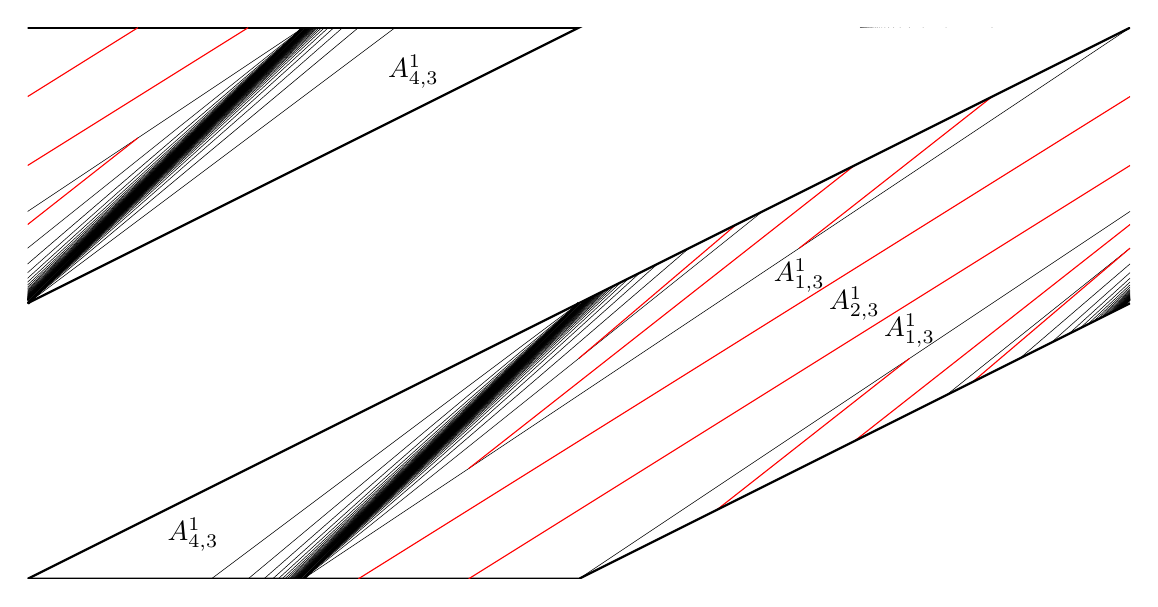
\begin{tikzpicture}[scale=1.4]
    
    \clip (0,5) rectangle (10,10);
        
        \foreach \k in {1,...,45}{
        % Blue in R3
                \draw[very thin] ({ (2*\k+2)*(7.5-7.5)/(2*\k+1)  }, { 7.5 })--({ (2*\k+2)*(10-7.5)/(2*\k+1)  }, { 10 });
        \draw[very thin] ({ 5+ (2*\k+2)*(5-7.5)/(2*\k+1)  }, { 5 })--({ 5+ (2*\k+2)*(7.5-7.5)/(2*\k+1) }, { 7.5 });
        % Red in R3/R4
        \draw[very thin] ({ 2.5 + (2*\k+1)*(5-5)/(2*\k)  }, { 5 })--({ 2.5 + (2*\k+1)*(10-5)/(2*\k)  }, { 10 });
        
         \draw[very thin] ({ 2.5  }, { 10 })--({ 2.5 - (2*\k+1)*(10-5)/(2*\k)  }, { 5 });
        
        \draw[very thin] ({ 12.5 + (2*\k+1)*(5-10)/(2*\k)  }, { 5 }) -- ({ 12.5 + (2*\k+1)*((30*\k+20)/(4*\k+2)-10)/(2*\k)  }, { (30*\k+20)/(4*\k+2) });
        }
        
        % Red green, n=2
        \draw[red] (30/4,70/8) -- (4,6);
        \draw[red] (70/8,150/16) -- (7,8);
        % Symmetries...
        \draw[red] (15-30/4,15-70/8) -- (15-5,15-190/28);
        \draw[red] (15-70/8,15-150/16) -- (15-7,15-8);
        
        
        % Top left corner...
        %% Red red
        %\draw[red](2.5,10) -- (0 , 50/6);
        %% Red green
        \draw[red] (1,9) -- (0,15-190/28);
        
        
        % Red green, n=3
        \draw[red] (5,7)--(90/14,230/28);
        % Symmetry
        \draw[red] (15-5,15-7)--(15-90/14,15-230/28);
        
        
        \fill[fill=white] (0,5) -- (10,10) -- (5,10) -- (0,7.5);
        \fill[fill=white] (10,5) -- (5,5) -- (10,7.5);
        
        \draw[thick] (0,10) -- (5,10) -- (0,7.5);
        \draw[thick] (0,5) -- (10,10);
        \draw[thick] (0,5) -- (5,5) -- (10,7.5); 
        
        
        % Red green, n=1
        \draw[red] (0,150/16) -- (1,10);
        \draw[red] (0,70/8) -- (2,10);
        \draw[red] (10,150/16) -- (3,5);
        \draw[red] (10,70/8) -- (4,5);
      
        \node at (7.5,7.5) {$A_{2,3}^1$};
        \node at (7,7.75) {$A_{1,3}^1$};
        \node at (8,7.25) {$A_{1,3}^1$};
     
         
        \node at (3.5,9.6) {$A_{4,3}^1$};
        
        \node at (5-3.5,15-9.6) {$A_{4,3}^1$};
    
    
        \draw[very thick] (0,7.5) -- (2.5,10);
        \draw[very thick] (2.5,5) -- (5,7.5);
      
      %\draw[very thick] (190/89,215/89) -- (230/89,190/89) -- (5-190/89,5-215/89) -- (5-230/89,5-190/89) -- (190/89,215/89);
      %\node at (230/89+0.15,190/89-0.05) {$Q$};
    \end{tikzpicture}
    }
    
    
    \caption{Partitions of the region $A_3$. Part (a) shows a partition into sets $A^k$ where $k$ is the escape time. Part (b) shows a subdivision into sets $A_{j,3}^k \subset A^k$ where $j$ is such that $H^k(A_{j,3}^k) \subset A_j$. Red lines in each $A^k$ are the preimages of the $A_1A_2$ boundary under $H^k$.}
    \label{fig:singSetConstruction}
\end{figure}

Now consider recurrence to $\sigma$ with return times greater than 1, the white regions of Figure \ref{fig:returnTime1}. Starting with $z \in A_3$, by the definition of $\sigma$, the return time $R(z;H,\sigma) = k+1$ where $k$ is the escape time $E(z;H,A_3)$. Figure \ref{fig:escapeTimes} shows a partition of $A_3$ into sets $A^k$ of constant escape time, bounded by the boundary preimages $H^{-k}(\partial A_3)$. Points in $A^k$ spend $k$ iterates in $A_3$ then escape via $A_1$, $A_2$, or $A_4$ and consequently return to $\sigma$. We partition each $A^k$ based on this escape path, shown as the red lines in Figure \ref{fig:escapeBehaviour}. The labelling $A_{j,i}^k$ is such that $A_{j,i}^k \subset A^k \subset A_i$ and $H^k(A_{j,i}^k) \subset A_j$. It transpires that when points escape after spending 4 or more iterates in $A_3$, they can only do so via $A_1$ or $A_4$. Similarly partitioning $A_2$ and combining with Figure \ref{fig:returnTime1} gives a partition of $\sigma$ into sets on which $DH_\sigma$ is constant. The boundaries of these partition elements are shown in Figure \ref{fig:HSigma} and constitutes, together with $\partial \sigma$, the singularity set $\mathcal{S}$ for $H_\sigma$. We remark that outside of the sets $\varsigma_2$, $\varsigma_3$ the Jacobian $DH_\sigma$ takes values in $\mathcal{M}$. Noting $H_\sigma(\varsigma_2) = H(\varsigma_2) \subset \sigma_3$ and $H_\sigma(\varsigma_3) = H(\varsigma_3) \subset \sigma_2$ we have that within $\varsigma_2$ the Jacobian of $H_\sigma^2$ is given by $M M_3$ for some $M \in \mathcal{M} \cup \{  M_2  \}$ and within $\varsigma_3$ it is given by $M M_2$ for some $M \in \mathcal{M} \cup \{  M_3  \}$. Hence, at almost every $z \in \sigma$ the Jacobian of $H_\sigma$ or $H_\sigma^2$ is some matrix from $\mathcal{M}$. We are now ready to establish non-uniform hyperbolicity.

\begin{proof}[Proof of Proposition \ref{prop:tentMap}]

The proof of Lemma \ref{lemma:itineraries} shows that almost every orbit $H^n(z)$ hits $\sigma$. Similar to LTMs, we can show that almost all of those then continue to return to $\sigma$ with some positive frequency $\alpha_z$. This follows straightforwardly from the fact that $H$ preserves the Lebesgue measure on $\tor$, a compact metric space, and $\sigma$ is measurable. A proof is given in Lemma 6.3.3 of \cite{sturman_mathematical_2006}, originally from \cite{burton_ergodicity_1980}. For large $n$ and a.e. $z$ the cardinality of $\{ 0 \leq i  \leq n - 1 \, | \, H^i(z) \in \sigma \}$ is roughly $\alpha_z n$, certainly
bounded below by $\alpha zn/2$\footnote{By a combinatorial argument, see \cite{sturman_mathematical_2006}.}. The cocycle $DH_z^n$ then contains as many applications of $DH_\sigma$. By the above, applying $DH_\sigma$ either completes a block from $\mathcal{M}$ or does so over the next iterate (the case where we land in $\varsigma_2,\varsigma_3$). At worst, then, we have roughly half as many blocks from $\mathcal{M}$ in $DH_z^n$ as we have returns to $\sigma$. Certainly this proportion is greater than a quarter, so $DH_z^n$ contains at least $\alpha_z n/8$ blocks from $\mathcal{M}$. Defining
\[ K = \inf_{\substack{M \in \mathcal{M}\\ v \in \mathcal{C}}} \frac{\| M v \|}{\| v \|}, \]
Lemma \ref{lemma:cone} gives $K>1$. Noting cone invariance, for any $v_0 \in \mathcal{C}$,
\begin{equation*}
\begin{split}
\frac{1}{n} \log \| DH_z^n v_0  \| & \geq \frac{1}{n} \log \left( K^{\frac{1}{8} \alpha_z n} \| v_0 \|  \right) \\
& = \frac{\alpha_z}{8} \log ( K) + \frac{1}{n} \log \| v_0 \|
\end{split}
\end{equation*}
so that $\chi(z,v_0) \geq \alpha_z \log (K) /8> 0$. We may then extend to non-zero Lyapunov exponents for general $v \neq 0$ using a particular form of Oseledets' theorem in two dimensions (Theorem 3.14 of \citealp{viana_lectures_2014}, see \citealp{myers_hill_exponential_2022}).
\end{proof}

